\documentclass{article}
\usepackage[T1]{fontenc}
\usepackage{lmodern}
\usepackage{graphicx}
\usepackage{amsmath,amssymb}
\usepackage[a4paper,margin=2cm]{geometry}
\usepackage[absolute,overlay]{textpos}
\setlength{\TPHorizModule}{1mm}
\setlength{\TPVertModule}{1mm}
\usepackage[indonesian]{babel}
\usepackage{hyperref}
\setlength{\emergencystretch}{2em}
\title{05-One-Time-Pad-(2026)}
\author{pdf\_ppt\_to\_latex}
\date{}

\begin{document}

% --- unit llm 1 ---
% === Halaman 1 (llm) ===

\begin{center}
Bahan kuliah IF4020 Kriptografi

\vspace{10mm}
\Huge \textcolor{red}{06 - One-Time Pad,}\
\Huge \textcolor{red}{Cipher yang Tidak Dapat Dipecahkan}\
\Huge \textcolor{red}{(Unbreakable Cipher)}

\vspace{136.62mm}

\vspace{10mm}
\Large Oleh: Rinaldi M

\vspace{10mm}
\large Program Studi Teknik Informatika\
Sekolah Teknik Elektro dan Informatika\
Institut Teknologi Bandung\
2026
\end{center}

% deskripsi: Foto tangan seseorang yang memegang sebuah buku kecil atau catatan berisi tabel angka-angka acak yang kemungkinan merupakan representasi dari kunci One-Time Pad.
% bbox normalisasi: [0.0600, 0.4900, 0.2300, 0.9500]
\begin{textblock*}{35.70mm}(12.60mm,145.53mm)
\noindent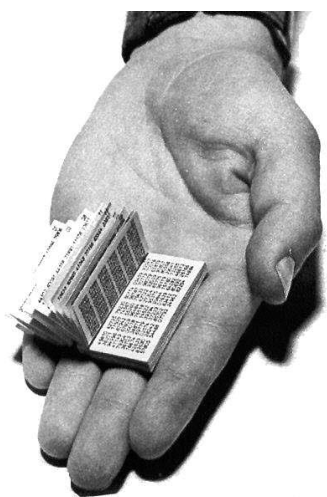
\includegraphics[width=35.70mm,height=136.62mm]{images/llm/page_001_img_01.png}%
\end{textblock*}

\newpage

% --- unit llm 2 ---
% === Halaman 2 (llm) ===

\section*{Pendahuluan}

\begin{itemize}
    \item \textcolor{red}{Unbreakable cipher} merupakan klaim yang dibuat oleh kriptografer terhadap algoritma kriptografi yang dirancangnya.
    \item Namun, kebanyakan algoritma yang sudah pernah dibuat orang adalah \textcolor{red}{breakable cipher}.
    \item Caesar Cipher, Vigenere Cipher, Playfair Cipher, Affine Cipher, Enigma Cipher, Hill Cipher, dll sudah kadaluarsa karena \textcolor{red}{breakable cipher}.
\end{itemize}

\newpage

% --- unit llm 3 ---
% === Halaman 3 (llm) ===

\begin{itemize}
    \item Apakah \textit{unbreakable cipher} memang benar-benar ada?
    Jawaban: ada!
    \item Apa syarat sebuah \textit{cipher} disebut \textit{unbreakable cipher}?
    Jawaban:
    \begin{enumerate}
        \item Kunci harus acak sejati (\textit{truly random}).
        \item Panjang kunci = panjang plainteks
        \item Kunci hanya boleh digunakan sekali, tidak boleh digunakan ulang untuk mengenkripsi pesan yang lain
    \end{enumerate}
    \item Acak sejati artinya tidak dapat diprediksi nilainya dan tidak dapat diulang kembali pembangkitannya. Ini berbeda dengan \textit{pseudo random} yang bisa diulang kembali pembangkitan nilai acak asalkan umpan (\textit{seed}) nya sama.
    \item Akibat 1 dan 2: plainteks yang sama tidak selalu menghasilkan cipherteks yang sama
\end{itemize}

\newpage

% --- unit llm 4 ---
% === Halaman 4 (llm) ===

\section*{One-Time Pad (OTP)}

\begin{itemize}
    \item Satu-satunya algoritma kriptografi sempurna aman (\textit{perfect secrecy}) sehingga tidak dapat dipecahkan adalah \textit{one-time pad (OTP)}.
    \item OTP ditemukan oleh Gilbert Vernam pada tahun 1917 dan kemudian secara matematis dibuktikan memiliki \textit{perfect secrecy} oleh Claude Shannon tahun 1949.
    \item OTP mengatasi kelemahan pada pada \textit{Vigenere Cipher}. \textit{Vigenere Cipher} mengulang penggunaan kunci secara periodik $\rightarrow$ mudah ditemukan dengan metode Kasiski.
    \item Pada OTP, panjang kunci = panjang plainteks, seluruh karakternya acak sejati
\end{itemize}

\vspace{5mm}

\begin{flushleft}
\textcolor{red}{\textbf{Plainteks:}} \texttt{otpadalahcipheryangtidakbisadipecahkan} \\
\textcolor{red}{\textbf{Kunci:}} \texttt{trjkdndkdwerylgrgdkopcegyhbdwjbtrfhgvk}
\end{flushleft}

\newpage

% --- unit llm 5 ---
% === Halaman 5 (llm) ===

\section*{Gilbert Vernam}

\vspace{139.89mm}

From Wikipedia, the free encyclopedia

\textbf{Gilbert Sandford Vernam} (April 3, 1890 -- February 7, 1960) was a Worcester Polytechnic Institute 1914 graduate and AT\&T Bell Labs engineer who, in 1917, invented an additive polyalphabetic stream cipher and later co-invented an automated one-time pad cipher. Vernam proposed a teleprinter cipher in which a previously prepared key, kept on paper tape, is combined character by character with the plaintext message to produce the ciphertext. To decipher the ciphertext, the same key would be again combined character by character, producing the plaintext. Vernam later worked for the Postal Telegraph Company, and became an employee of Western Union when that company acquired Postal in 1943. His later work was largely with automatic switching systems for telegraph networks.

\vspace{10mm}

\begin{tabular}{|l|l|}
\hline
\multicolumn{2}{|c|}{\textbf{Gilbert Vernam}} \\ \hline
\textbf{Born} & April 3, 1890 \\ \hline
\textbf{Died} & February 7, 1960 (aged 69) \\ \hline
\textbf{Alma mater} & Worcester Polytechnic Institute \\ \hline
\textbf{Occupation} & Cryptographer \\ \hline
\end{tabular}

% deskripsi: Foto potret hitam putih Gilbert Vernam
% bbox normalisasi: [0.7700, 0.2030, 0.9520, 0.6740]
\begin{textblock*}{38.22mm}(161.70mm,60.29mm)
\noindent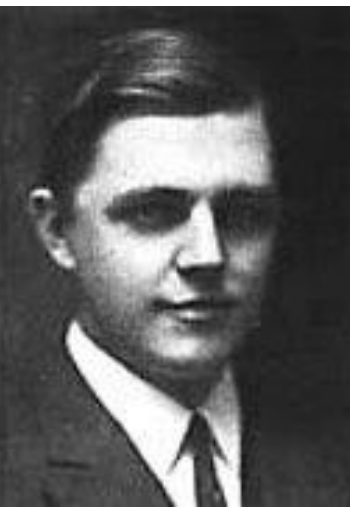
\includegraphics[width=38.22mm,height=139.89mm]{images/llm/page_005_img_01.png}%
\end{textblock*}

\newpage

% --- unit llm 6 ---
% === Halaman 6 (llm) ===

\begin{itemize}
  \item \textit{One-time pad} (\textit{pad} = kertas bloknot) berisi deretan huruf-huruf kunci yang dibangkitkan secara acak.
\end{itemize}

\vspace{10mm}

Sumber: https://www.cryptomuseum.com/crypto/otp/index.htm

% deskripsi: Foto tangan seseorang yang sedang memegang buku catatan (pad) yang berisi tabel huruf acak untuk metode enkripsi one-time pad.
% bbox normalisasi: [0.2500, 0.2600, 0.7300, 0.8200]
\begin{textblock*}{100.80mm}(52.50mm,77.22mm)
\noindent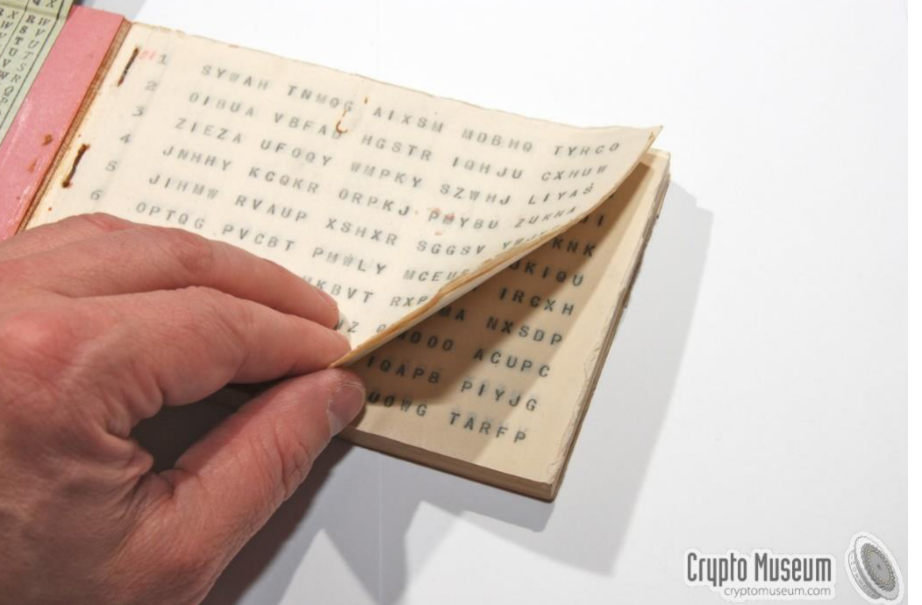
\includegraphics[width=100.80mm,height=166.32mm]{images/llm/page_006_img_01.png}%
\end{textblock*}

\newpage

% --- unit llm 7 ---
% === Halaman 7 (llm) ===

CIHJT UUHML FRUGC ZIBGD BQPNI PDNJG LPLLP YJYXM\\
DCXAC JSJUK BIOYT MWQPX DLIRC BEXYK VKIMB TYIPE\\
UOLYQ OKOXH PIJKY DRDBC GEFZG UACKD RARCD HBYRI\\
DZJYO YKAIE LIUYW DFOHU IOHZV SRNDD KPSSO JMPQT\\
MHQHL OHQQD SMHNP HHOHQ GXRPJ XBXIP LLZAA VCMOG\\
AWSSZ YMFNI ATMON IXPBY FOZLE CVYSJ XZGPU CTFQY\\
HOVHU OCJGU QMWQV OIGOR BFHIZ TYFDB VBRMN XNLZC

\newpage

% --- unit llm 8 ---
% === Halaman 8 (llm) ===

\begin{itemize}
    \item Pengirim dan penerima pesan memiliki salinan (\textit{copy}) \textit{pad} yang sama.
    \item Satu \textit{pad} hanya digunakan sekali (\textit{one-time}) saja untuk mengenkripsi pesan\\
    $\rightarrow$ itulah mengapa dinamakan \textit{one-time pad}.
    \item Sekali \textit{pad} telah digunakan, ia dihancurkan supaya tidak dipakai kembali untuk mengenkripsi pesan yang lain\\
    $\rightarrow$ menyulitkan kriptanalisis
\end{itemize}

\newpage

% --- unit llm 9 ---
% === Halaman 9 (llm) ===

\vspace{92.07mm}

\vspace{30mm}
\begin{itemize}
    \item Aturan enkripsi dan dekripsi yang digunakan persis sama seperti pada \textit{Vigenere Cipher}, bedanya tidak ada perulangan kunci secara periodik.
    \item Enkripsi: $C = (P + K) \pmod{26}$
    
    Contoh ($P = \text{'o'}$, $K = \text{'t'}$): $C = (\text{'o'} + \text{'t'}) \pmod{26} = (14 + 19) \pmod{26} = 33 \pmod{26} = 7 = \text{'H'}$
    
    \item Dekripsi: $P = (C - K) \pmod{26}$
    
    Contoh ($C = \text{'H'}$, $K = \text{'t'}$): $P = (\text{'H'} - \text{'t'}) \pmod{26} = (7 - 19) \pmod{26} = -12 \pmod{26} = 14 = \text{'o'}$
\end{itemize}

% deskripsi: Tabel konversi huruf ke angka dan contoh proses enkripsi teks menggunakan metode cipher dengan plaintext, kunci, dan ciphertexts.
% bbox normalisasi: [0.3900, 0.0000, 0.9800, 0.3100]
\begin{textblock*}{123.90mm}(81.90mm,0.00mm)
\noindent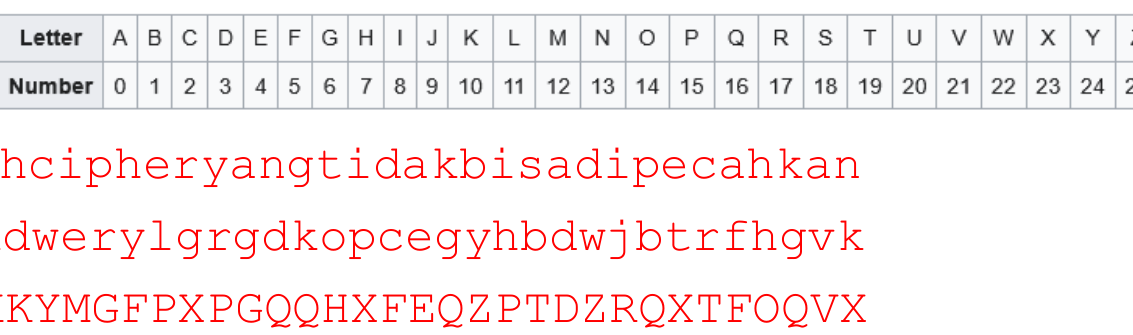
\includegraphics[width=123.90mm,height=92.07mm]{images/llm/page_009_img_01.png}%
\end{textblock*}

\newpage

% --- unit llm 10 ---
% === Halaman 10 (llm) ===

\begin{itemize}
    \item \textbf{Contoh 1:}

    Plainteks: \texttt{onetimepad}\
    Kunci: \texttt{tbfrgfarfm}

    Misalkan $A = 0, B = 1, ..., Z = 25$.

    cipherteks: \texttt{HOJKOREGHP}

    yang dalam hal ini diperoleh sebagai berikut:
    \[
    \begin{aligned}
    ('o' + 'T') \pmod{26} &= H \\
    ('n' + 'B') \pmod{26} &= O \\
    ('e' + 'F') \pmod{26} &= J, \text{ dst}
    \end{aligned}
    \]
\end{itemize}

\newpage

% --- unit llm 11 ---
% === Halaman 11 (llm) ===

\begin{itemize}
    \item[$\bullet$] \textbf{Contoh 2:}
\end{itemize}

\begin{tabular}{ll}
    Plainteks: & \texttt{nantimalamsayatunggukamudidepanwarungkopi} \\
    Kunci: & \texttt{gtrskncvbrwpoatqljfmxr pjsrzfoltfbtmaedpvy} \\
    Cipherteks: & \texttt{TTELSZCGBDOPMAMKYPLGHTDJMAUDDLSDTSGNKNDKG}
\end{tabular}

\newpage

% --- unit llm 12 ---
% === Halaman 12 (llm) ===

\section*{Demo One Time Pad Onlie}

\vspace{180.28mm}

\begin{itemize}
    \item \url{https://www.cachesleuth.com/onetimepad.html}
\end{itemize}

\vspace{10mm}

% deskripsi: Screenshot halaman web tool 'One Time Pad Cipher' yang menunjukkan area input untuk Plaintext, pilihan alfabet, dan Encryption Key.
% bbox normalisasi: [0.1350, 0.3760, 0.7360, 0.9830]
\begin{textblock*}{126.21mm}(28.35mm,111.67mm)
\noindent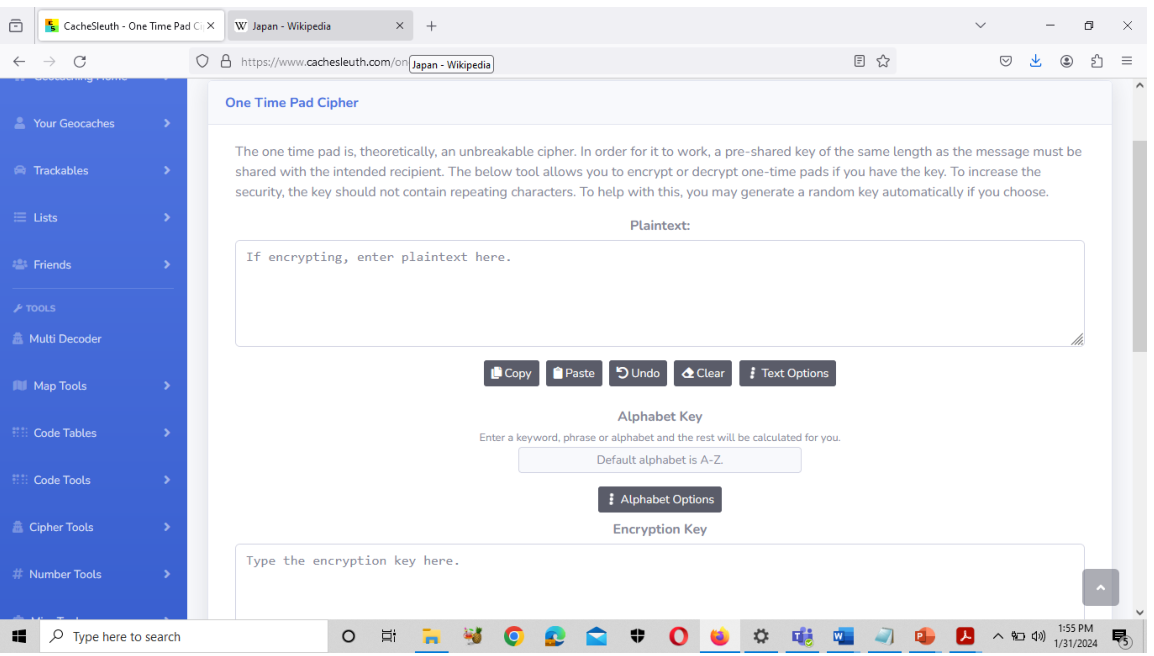
\includegraphics[width=126.21mm,height=180.28mm]{images/llm/page_012_img_01.png}%
\end{textblock*}

\newpage

% --- unit llm 13 ---
% === Halaman 13 (llm) ===

\begin{itemize}
    \item Kunci untuk OTP harus seluruhnya acak sejati dan sepanjang pesan.
    \item Bagaimana jika kunci diambil dari teks yang panjang (misalnya tulisan di dalam novel, buku, berita, dan sebagainya)?
    \begin{itemize}
        \item ini bukan lagi OTP (sebab tulisan di buku/novel/berita bukan acak)
        \item tidak menghasilkan \textit{perfect secrecy}
        \item dapat dipecahkan
    \end{itemize}
    \item Kunci di dalam OTP hanya dipakai sekali dan tidak pernah digunakan kembali. Bagaimana jika kunci dipakai untuk kedua kalinya?
    \begin{itemize}
        \item ia bukan lagi \textit{one-time pad}, tetapi \textit{two-time pad}
        \item tidak aman
    \end{itemize}
\end{itemize}

\newpage

% --- unit llm 14 ---
% === Halaman 14 (llm) ===

\begin{itemize}
    \item[$\bullet$] \textbf{OTP ini tidak dapat dipecahkan karena:}
    \begin{enumerate}
        \item Kunci OTP (acak) + plainteks (tidak acak) = cipherteks (acak)
        
        \begin{align*}
            \text{Enkripsi: } C &= (P + K) \pmod{26} \\ 
            \text{Dekripsi: } P &= (C - K) \pmod{26}
        \end{align*}
        
        \item Hanya terdapat satu kunci yang memetakan plainteks ke cipherteks, begitu juga sebaliknya
        \begin{itemize}
            \item[$\rightarrow$] fungsi $C = (P + K) \pmod{26}$ adalah pemetaan satu-ke-satu (\textit{one-to-one}).
            \item[$\rightarrow$] artinya, untuk sembarang plainteks dan cipherteks hanya ada satu kunci yang memetakannya satu sama lain
            \item[$\rightarrow$] Akibatnya, jika kriptanalis mencoba mendekripsi cipherteks dengan beberapa kunci berbeda ada kemungkinan menghasilkan beberapa plainteks yang bermakna, sehingga kriptanalis kesulitan menentukan plainteks mana yang benar.
        \end{itemize}
    \end{enumerate}
\end{itemize}

\newpage

% --- unit llm 15 ---
% === Halaman 15 (llm) ===

\begin{itemize}
  \item \textbf{Contoh 3:} Misalkan kriptanalis mencoba kunci \texttt{LMCCAWAAZD} untuk mendekripsi cipherteks \texttt{HOJKOREGHP} \\
  Plainteks yang dihasilkan: \texttt{SALMONEGGS} \quad (telur ikan Salmon)
  
  \vspace{5mm}
  
  Bila ia mencoba kunci: \texttt{ZDVUZOEYEO} \\
  Plainteks yang dihasilkan: \texttt{GREENFIELD} \quad (lapangan hijau)
  
  \vspace{5mm}
  
  Kriptanalis: ??????? Kunci mana yang benar? (bingung sendiri $\smiley$)
  
  \vspace{5mm}
  
  \item Contoh ini menunjukkan bahwa untuk sembarang plainteks dan cipherteks hanya ada satu kunci yang memetakannya satu sama lain.
\end{itemize}

\newpage

% --- unit llm 16 ---
% === Halaman 16 (llm) ===

\begin{itemize}
    \item Sebagai latihan, misalkan diberikan sebuah cipherteks:
    \begin{center}
        \texttt{TLCYKUMGDFAWTZVOYKLENSZZHYZRW}
    \end{center}
\end{itemize}

temukan kunci yang menghasilkan plainteks:
\begin{center}
    \texttt{mr johnson left his house last night}
\end{center}

lalu temukan kunci lain yang menghasilkan plainteks
\begin{center}
    \texttt{i saw the mysterious plane behind me}
\end{center}

\newpage

% --- unit llm 17 ---
% === Halaman 17 (llm) ===

\begin{itemize}
  \item Pembuktian
  
  \"kunci OTP (acak) + plainteks (tidak acak) = cipherteks (acak)\" \\
  sebagai berikut:\
  Misalkan:\n  \[ C = (P + K) \pmod{26} \]
  dengan $K$ dipilih secara uniform:\n  \[ P(K = k) = \frac{1}{26}, \quad k = 0, 1, \dots, 25. \]
  Untuk setiap nilai plainteks tertentu $P = p$, pemetaan
  \[ C = (P + K) \pmod{26} \]
  merupakan pemetaan satu-ke-satu dari semua kemungkinan $K$ ke semua kemungkinan $C$.\
  Akibatnya:\n  \[ P(C = c \mid P = p) = \frac{1}{26} \]
  untuk setiap $c$ (yaitu: $P(C = \text{'a'}) = P(C = \text{'b'}) = \dots = P(C = \text{'z'}) = \frac{1}{26}$)
\end{itemize}

\newpage

% --- unit llm 18 ---
% === Halaman 18 (llm) ===

\vspace{89.40mm}

\section*{Perfect Secrecy}

\begin{itemize}
    \item \textit{Perfect secrecy}: Cipherteks tidak menyediakan informasi apapun tentang plainteks maupun kunci.
    \item Pada tahun 1949, Claude Shannon dari Laboratorium Bell membuktikan bahwa OTP memiliki \textit{perfect secrecy}. Ia menulis pembuktian tsb di dalam makalahnya:
    
    \textcolor{red}{"Shannon, C. E. (1949). Communication theory of secrecy systems. Bell System Technical Journal, 28(4), 656--715."}
    
    \item Menurut Shannon, suatu sistem memiliki \textit{perfect secrecy} apabila setelah penyerang memperoleh cipherteks, informasi mengenai plainteks tidak bertambah. Secara matematis, kondisi tersebut dinyatakan sebagai:
    
    \[ P(P = p \mid C = c) = P(P = p) \]
    
    Artinya, probabilitas suatu plainteks tertentu tetap sama sebelum maupun setelah cipherteks diamati
\end{itemize}

% deskripsi: Foto potret Claude Shannon
% bbox normalisasi: [0.8580, 0.0240, 0.9760, 0.3250]
\begin{textblock*}{24.78mm}(180.18mm,7.13mm)
\noindent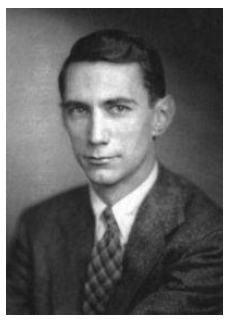
\includegraphics[width=24.78mm,height=89.40mm]{images/llm/page_018_img_01.png}%
\end{textblock*}

\newpage

% --- unit llm 19 ---
% === Halaman 19 (llm) ===

\begin{center}
\textbf{Communication Theory of Secrecy Systems*}

By C. E. SHANNON
\end{center}

\section*{1 INTRODUCTION AND SUMMARY}

The problems of cryptography and secrecy systems furnish an interesting application of communication theory$^1$. In this paper a theory of secrecy systems is developed. The approach is on a theoretical level and is intended to complement the treatment found in standard works on cryptography$^2$. There, a detailed study is made of the many standard types of codes and ciphers, and of the ways of breaking them. We will be more concerned with the general mathematical structure and properties of secrecy systems.

The treatment is limited in certain ways. First, there are three general types of secrecy system: (1) concealment systems, including such methods as invisible ink, concealing a message in an innocent text, or in a fake covering cryptogram, or other methods in which the existence of the message is concealed from the enemy; (2) privacy systems, for example speech inversion, in which special equipment is required to recover the message; (3) \"true\" secrecy systems where the meaning of the message is concealed by cipher, code, etc., although its existence is not hidden, and the enemy is assumed to have any special equipment necessary to intercept and record the transmitted signal. We consider only the third type---concealment system are primarily a psychological problem, and privacy systems a technological one.

Secondly, the treatment is limited to the case of discrete information where the message to be enciphered consists of a sequence of discrete sym-

\newpage

% --- unit llm 20 ---
% === Halaman 20 (llm) ===

\section*{Kelemahan OTP}

\begin{itemize}
    \item Meskipun OTP menawarkan keamanan yang sempurna, tetapi ia tidak umum digunakan dalam aplikasi praktis (aplikasi komersil maupun aplikasi lainnya).
    \item Alasan:
    \begin{enumerate}
        \item Tidak sangkil, karena panjang kunci = panjang pesan. \\
        Makin panjang pesan, makin besar ukuran kuncinya. Butuh komputasi yang berat untuk membangkitkan milyaran karakter-karakter yang benar-benar acak. Untuk pesan yang sangat panjang atau komunikasi yang berlangsung terus-menerus, kebutuhan kuncinya menjadi sangat besar.
        \item Karena kunci dibangkitkan harus benar-benar acak (\textit{truly random}), maka 'tidak mungkin' pengirim dan penerima membangkitkan kunci acak yang sama secara simultan (bersamaan).
    \end{enumerate}
\end{itemize}

\newpage

% --- unit llm 21 ---
% === Halaman 21 (llm) ===

\begin{itemize}
  \item Untuk menggunakan OTP, pengirim dan penerima harus menyepakati kunci yang digunakan, kunci harus sepanjang pesan, dan hanya boleh digunakan sekali.
  \item Hal ini sulit dilakukan secara praktek.
  \item \textit{OTP} hanya dapat digunakan jika tersedia saluran komunikasi kedua yang sangat aman untuk mengirim kunci.
  \item Saluran kedua ini tidak boleh sama dengan saluran untuk mengirim pesan.
  \item Saluran kedua ini umumnya lambat dan mahal (misalnya lewat jalur darat, memakai kurir terpercaya dan tidak bisa dikenali).
  \item Atau, kunci dikirim pada saluran yang sama dengan saluran pengiriman pesan tetapi pada waktu yang berbeda dengan pengiriman pesan.
\end{itemize}

\newpage

% --- unit llm 22 ---
% === Halaman 22 (llm) ===

\begin{itemize}
    \item OTP Tidak cocok untuk komunikasi dinamis. Bayangkan untuk komunikasi modern seperti:
    \begin{itemize}
        \item WhatsApp
        \item HTTPS
        \item VPN
        \item cloud storage
        \item email
        \item komunikasi IoT, dll
    \end{itemize}
    data yang dikirim terus berubah, perangkat bisa berganti, pengguna bisa \textit{offline}, dan pesan memiliki ukuran yang berbeda-beda.
    \vspace{5mm}
    \item Dengan OTP, setiap tambahan data membutuhkan tambahan kunci yang benar-benar acak dan belum pernah digunakan. Ini membuat manajemen kunci menjadi sangat berat.
\end{itemize}

\newpage

% --- unit llm 23 ---
% === Halaman 23 (llm) ===

\begin{itemize}
    \item OTP pernah digunakan oleh mata-mata (\textit{spy}) selama Perang Dunia II
\end{itemize}

\vspace{80mm}

\textcolor{red}{\centering Pejabat eksekutif operasi khusus dari Inggris memperlihatkan syal yang bertuliskan kunci OTP selama PD II}

\vspace{10mm}

\begin{flushright}
\textcolor{red}{Sumber: John H Reif, History of Computing, Duke University}
\end{flushright}

% deskripsi: Foto seorang pria yang memegang selembar kain atau syal yang berisi teks terenkripsi (one-time pad) yang digunakan oleh mata-mata Perang Dunia II.
% bbox normalisasi: [0.1440, 0.2000, 0.5670, 0.8400]
\begin{textblock*}{88.83mm}(30.24mm,59.40mm)
\noindent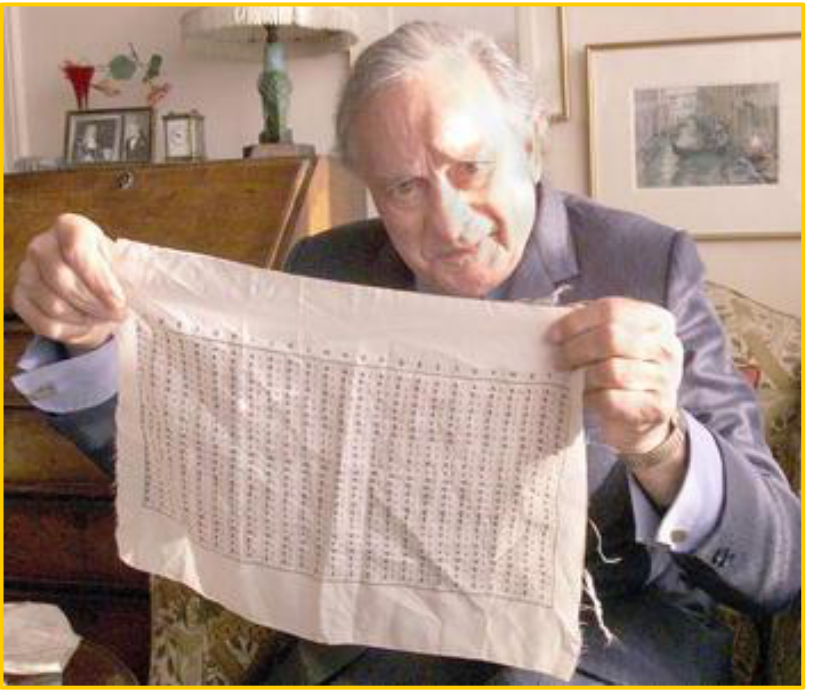
\includegraphics[width=88.83mm,height=190.08mm]{images/llm/page_023_img_01.png}%
\end{textblock*}

\newpage

% --- unit llm 24 ---
% === Halaman 24 (llm) ===

\vspace{173.45mm}

\textcolor{red}{\textbf{Penggunaan OTP pada perang dingin antara AS dan Uni Soviet}}

\vspace{238.79mm}

\textcolor{red}{\textbf{The Moscow--Washington hotline [1963]:}}
\begin{itemize}
    \item Komunikasi antara AS dan Uni Soviet menggunakan hotline komunikasi langsung antara pemimpin AS dan Uni Soviet.
    \item Hotline difasilitasi dengan peralatan OTP yang bernama ITT Intelex Teletype L015
\end{itemize}

\begin{itemize}
    \item ITT Intelex Teletype dikembangkan setelah krisis rudal Cuba untuk menghindari perang nuklir
\end{itemize}

\vspace{10mm}

\begin{itemize}
    \item \textcolor{red}{\textbf{ITT Intelex Teletype mengenkripsi pesan menggunakan OTP}}
    \begin{itemize}
        \item Kunci \textit{one-time pad} disimpan di dalam pita magnetic yang diterbangkan antara Washington DC dan Moscow.
    \end{itemize}
\end{itemize}

\vspace{10mm}

Sumber: John H Reif, History of Computing, Duke University

% deskripsi: Foto mesin ITT Intelex Teletype L015 yang digunakan untuk hotline Moskow-Washington.
% bbox normalisasi: [0.6970, 0.0000, 0.9260, 0.5840]
\begin{textblock*}{48.09mm}(146.37mm,0.00mm)
\noindent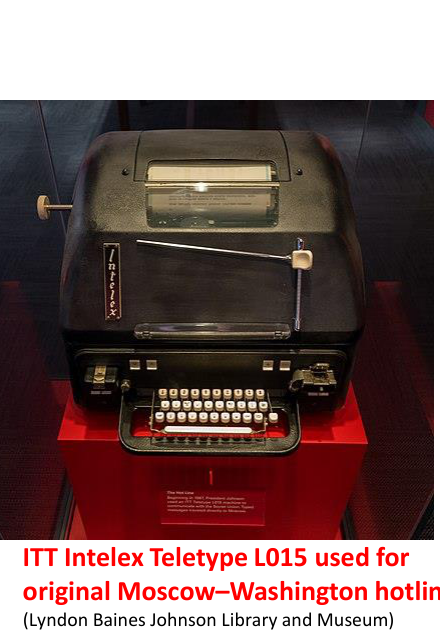
\includegraphics[width=48.09mm,height=173.45mm]{images/llm/page_024_img_01.png}%
\end{textblock*}

% deskripsi: Foto udara gedung Pentagon di Arlington County, Virginia, AS.
% bbox normalisasi: [0.5020, 0.6410, 0.6680, 0.8950]
\begin{textblock*}{34.86mm}(105.42mm,190.38mm)
\noindent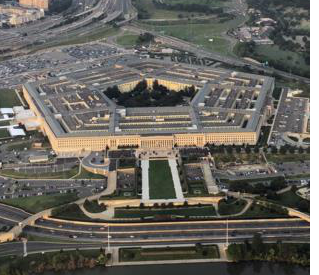
\includegraphics[width=34.86mm,height=75.44mm]{images/llm/page_024_img_02.png}%
\end{textblock*}

% deskripsi: Foto gedung Kremlin di Moskow, Rusia.
% bbox normalisasi: [0.7730, 0.6410, 0.9710, 0.8950]
\begin{textblock*}{41.58mm}(162.33mm,190.38mm)
\noindent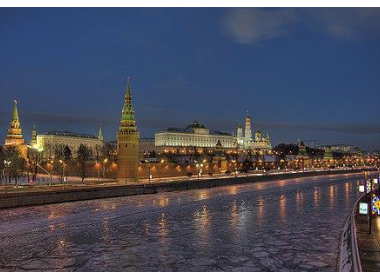
\includegraphics[width=41.58mm,height=75.44mm]{images/llm/page_024_img_03.png}%
\end{textblock*}

% deskripsi: Panah merah dua arah yang menunjukkan komunikasi antara Pentagon dan Kremlin.
% bbox normalisasi: [0.0600, 0.1080, 0.9400, 0.9120]
\begin{textblock*}{184.80mm}(12.60mm,32.08mm)
\noindent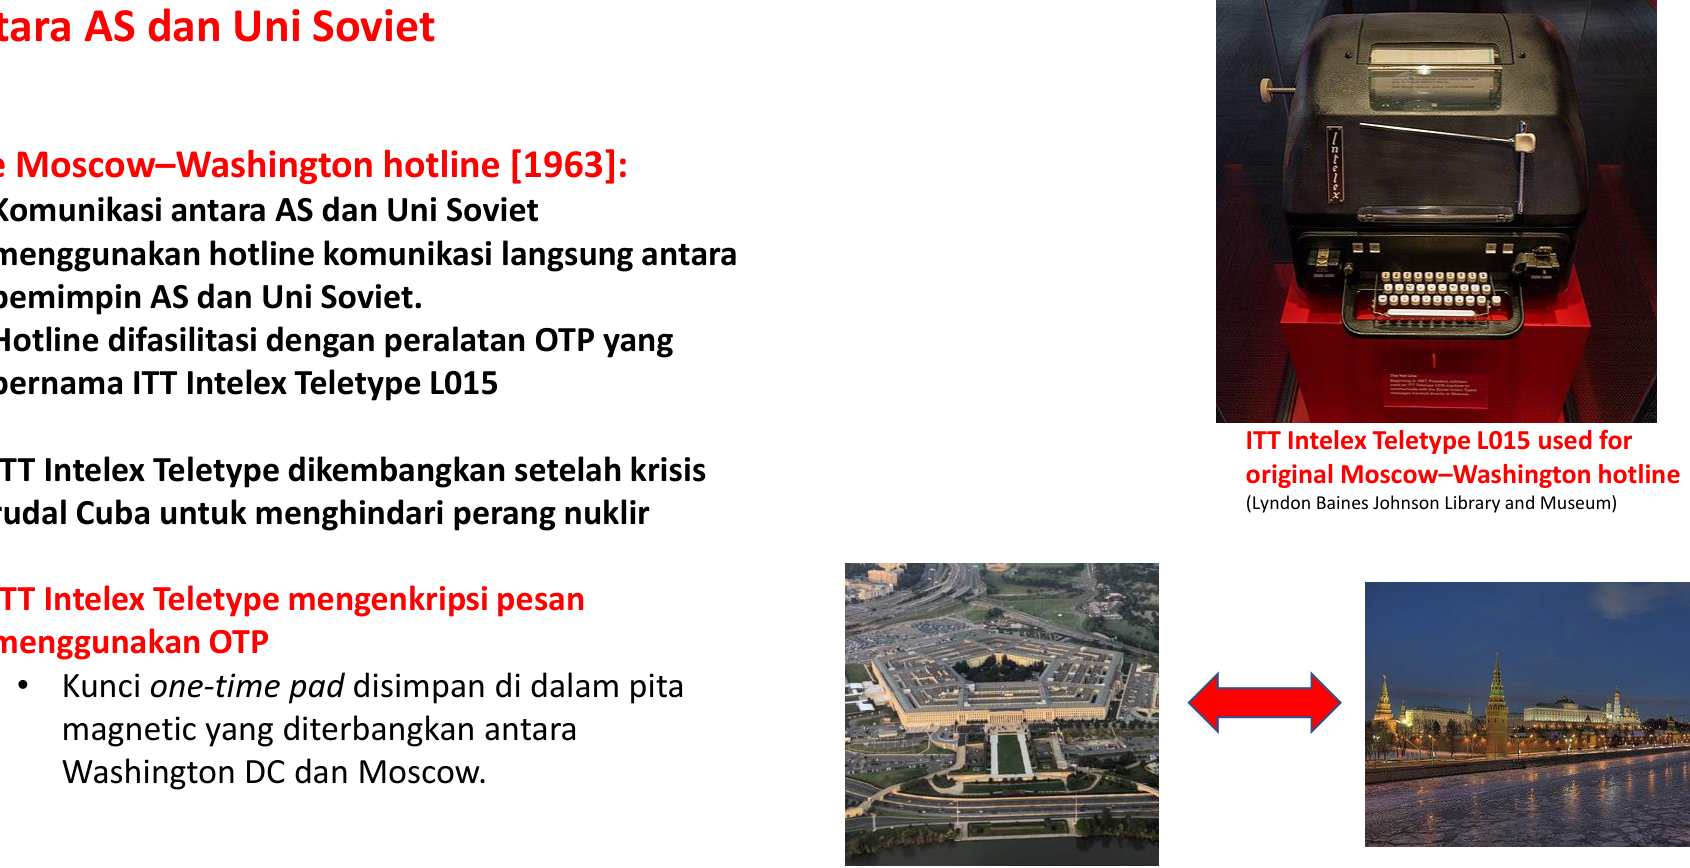
\includegraphics[width=184.80mm,height=238.79mm]{images/llm/page_024_img_04.png}%
\end{textblock*}

% bbox perkiraan otomatis: Panah merah dua arah yang menunjukkan komunikasi antara Pentagon dan Kremlin.

\newpage

% --- unit llm 25 ---
% === Halaman 25 (llm) ===

\begin{itemize}
  \item As a practical person, I've observed that one-time pads are theoretically unbreakable, but practically very weak. By contrast, conventional ciphers are theoretically breakable, but practically strong." - \textbf{Steve Bellovin}
\end{itemize}

\end{document}
